\chapter{関連研究}
\label{chap:kanren}

本章では楽譜関連研究を紹介し、それらの特徴や本研究との関連性について示す。

\newpage

\section{主要な研究領域}
楽譜に関連する主要な研究領域を紹介する。

\begin{enumerate}
  \item スコアアラインメント\\
  楽譜上のどの部分を演奏しているのか認識するためのスコアアラインメント技術が研究されている\cite{online}\cite{learning}\cite{coupled}\cite{automatic}。
  応用例として計算機による伴奏システム\cite{muens}\cite{mysong}、音楽鑑賞サポートシステム\cite{orchestra}、楽器練習サポートシステムなどが挙げられる\cite{tutor}。
  \item ジェスチャー楽譜入力インターフェース\\
  ジェスチャーを利用した楽譜入力インターフェースが提案されている\cite{notepad}\cite{pen}\cite{sssp}。
  これにより、計算機上でペンやポインティングデバイスを使って、楽譜を手書き入力することができる。
  \item 楽譜認識/再生システム\\
  画像から楽譜情報を読み取るための楽譜認識技術が研究されている\cite{optical}\cite{early}\cite{symbol}。
  これを応用して、カメラを搭載したデバイスによって印刷された楽譜を再生するシステムが提案されている\cite{onnote}\cite{gocen}。
\end{enumerate}

\section{楽譜編集/閲覧システム}
一般的に利用されている楽譜システムとは異なる、紙の楽譜の再現にとどまらない特徴を持った楽譜編集/閲覧システムを紹介する。

\subsection{BRASS}
Watanabeらが提案したBRASS\cite{Watanabe}(図\ref{brass})は、楽曲の全体構造を把握しながら楽譜を閲覧できるインタフェースによって、楽曲学習を支援する。
複数ページにまたがる規模の大きな楽譜では楽曲全体を把握するのが困難であるが、楽譜を圧縮表示し、音符の数やテンポの大小といったパラメータを濃淡や色によって可視化することで解決している。
ここで利用されている、空間を歪ませて注目部分を拡大表示する可視化手法はフォーカス+コンテクスト表示と呼ばれている。
本研究ではフォーカス+コンテクスト表示のような可視化の工夫は行っていないが、楽曲理解のために必要なテキスト/マルチメディアを自在に埋め込めることから、学習支援にも利用できる。

\begin{figure}[H]
\centering
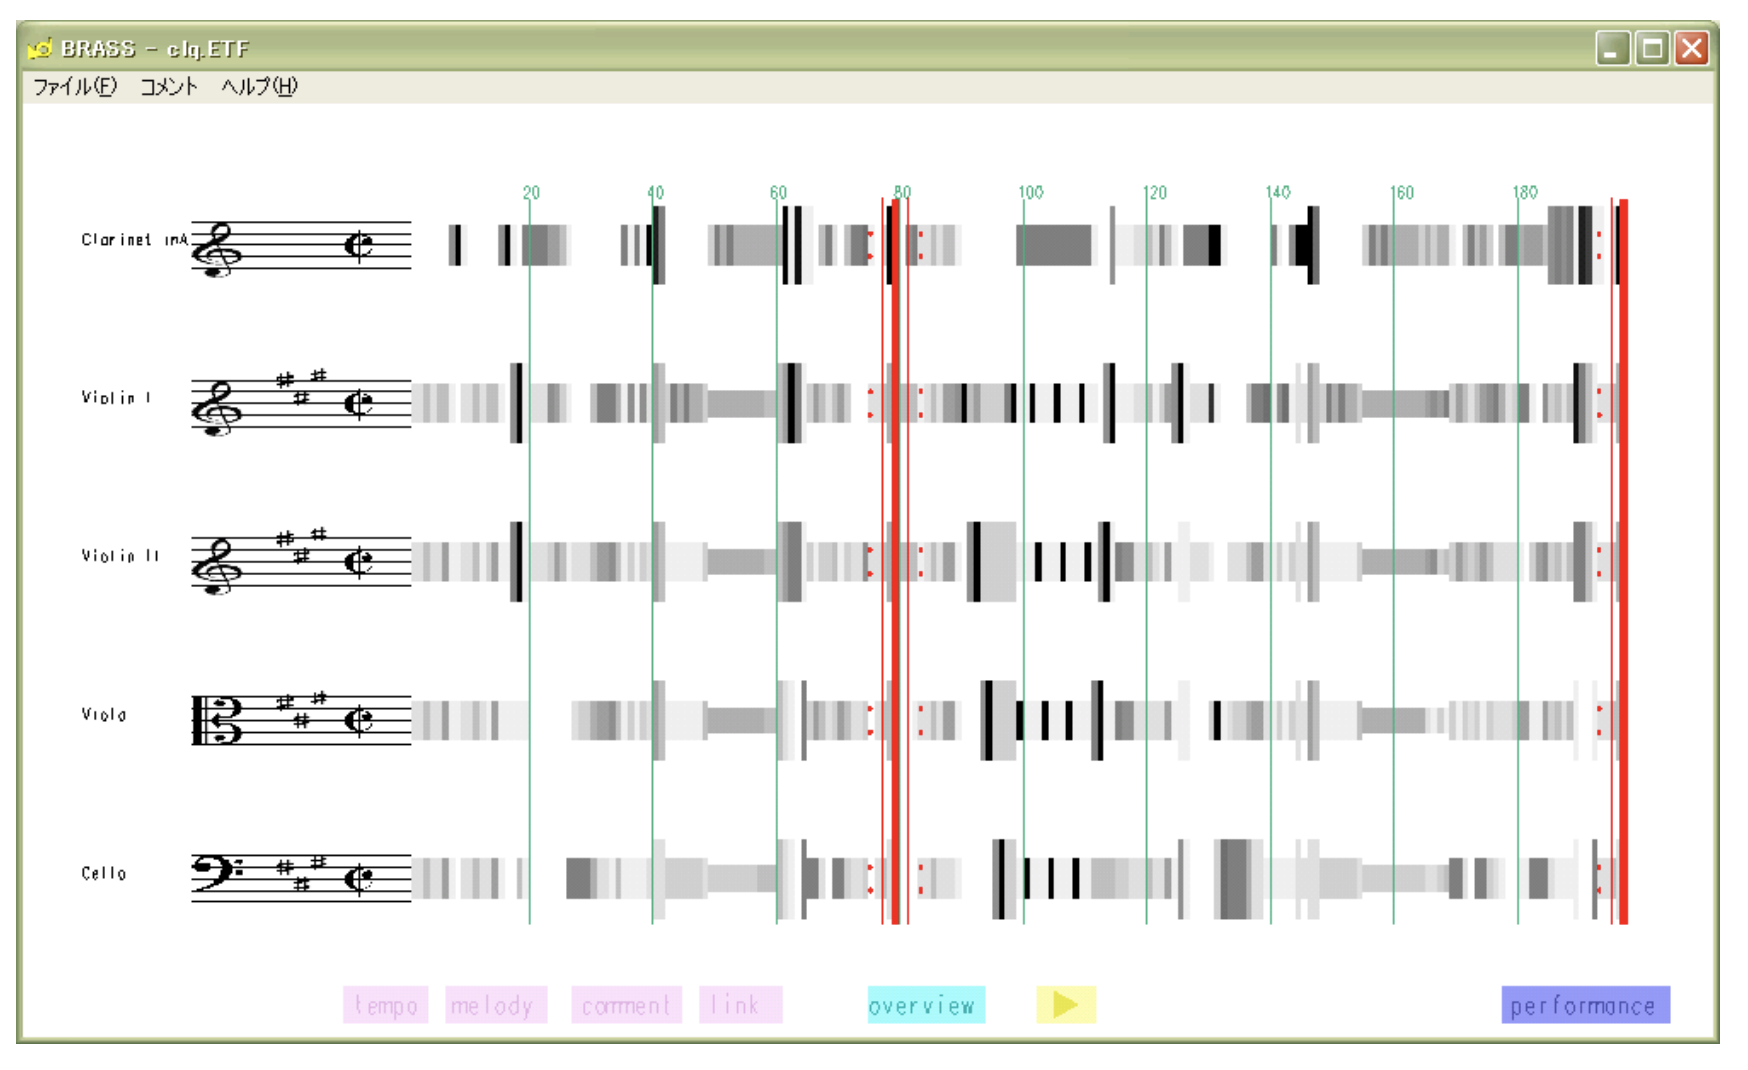
\includegraphics[width=10cm]{images/brass.png}
\caption{BRASSの画面}
\label{brass}
\end{figure}

\subsection{WIKI: :SCORE}
Almeidaらが提案したWIKI: :SCORE\cite{Almeida}(図\ref{wikiscore})は、Wiki上で楽譜の共同編集を行えるシステムである。
ABCによって楽譜を編集し、PDF/画像/音声といった各種フォーマット出力することができる。
複数パート/セクションを持つ規模の大きな楽譜の編集は大変な作業であるが、共同編集や楽譜の出力を行えることで、複数人で協力して実行することが可能である。
WikiとABCによるシステムであることからハイパー楽譜システムに設計が近いが、以下の点で異なっている。
\begin{itemize}
\item 共同編集のみを問題にしている
\item 編集環境がWYSIWYGでない
\item 楽譜専用のWikiである
\end{itemize}

\begin{figure}[H]
\centering
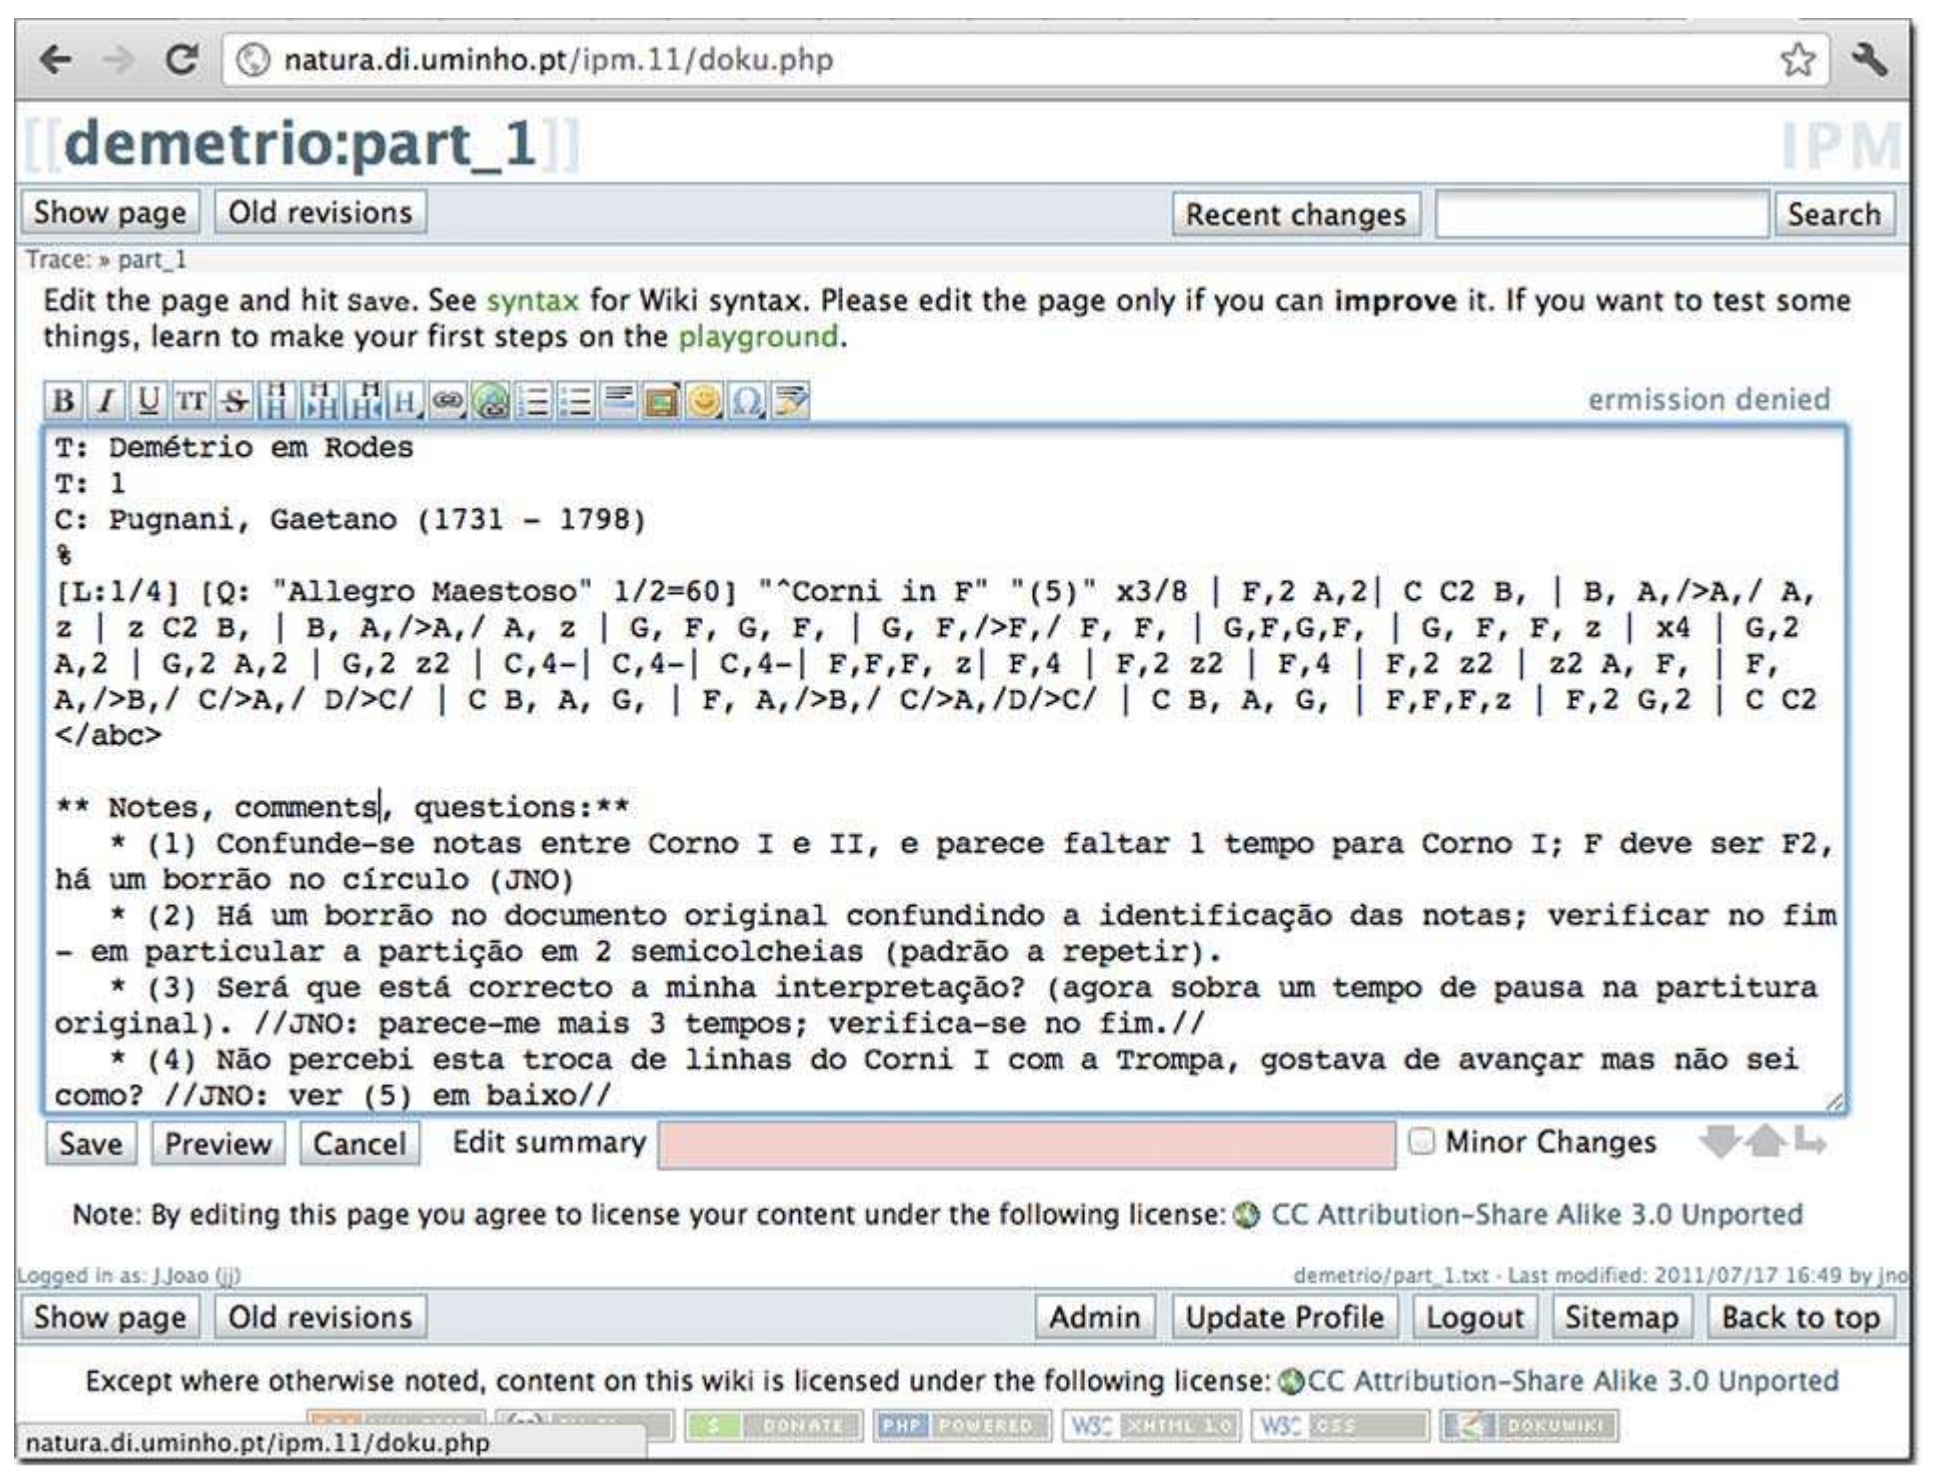
\includegraphics[width=10cm]{images/wikiscore.png}
\caption{WIKI: :SCOREの画面}
\label{wikiscore}
\end{figure}

\section{楽譜記述言語}
楽譜記述言語は楽譜をベースとした楽曲を記録・共有する目的で利用されており、本研究で利用しているABC記譜法もその1つである。
本節ではABC以外に広く利用されているものを解説する。
比較のために、図\ref{cdef}の楽譜を記述する各言語の例を示す。
ソースコード\ref{abcdef}はABCにおける記述例である。

\begin{figure}[H]
\centering
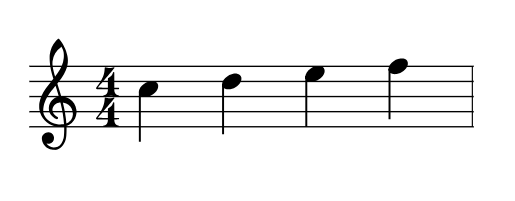
\includegraphics[width=5cm]{images/cdef.png}
\caption{「ドレミファ」の譜例}
\label{cdef}
\end{figure}

\begin{lstlisting}[caption=ABCにおける図\ref{cdef}の楽譜の記述例, label=abcdef]
M:4/4
L:1/4
cdef|
\end{lstlisting}

\subsection{MusicXML}
MusicXML\cite{XML}はXML形式の楽譜記述言語で、音符や小節といった音楽的要素が階層的に記述される。
各種楽譜作成ソフトでもMusicXMLによるインポート/エクスポートがサポートされており、楽譜データのやりとりに広く利用されている。
\begin{lstlisting}[caption=MusicXMLにおける図\ref{cdef}の楽譜の記述例(一部), label=xml]
<score-partwise>
  <part-list>
    <score-part id="P1">
      <part-name>Piano</part-name>
    </score-part>
  </part-list>
  <part id="P1">
    <measure number="1">
      <attributes>
        <divisions>1</divisions>
        <key>
          <fifths>0</fifths>
        </key>
        <time>
          <beats>4</beats>
          <beat-type>4</beat-type>
        </time>
        <clef>
          <sign>G</sign>
          <line>2</line>
        </clef>
      </attributes>
      <note>
        <pitch>
          <step>C</step>
          <octave>5</octave>
        </pitch>
        <duration>1</duration>
        <type>quarter</type>
      </note>
      <note>
        <pitch>
          <step>D</step>
          <octave>5</octave>
        </pitch>
        <duration>1</duration>
        <type>quarter</type>
      </note>
      <note>
        <pitch>
          <step>E</step>
          <octave>5</octave>
        </pitch>
        <duration>1</duration>
        <type>quarter</type>
      </note>
      <note>
        <pitch>
          <step>F</step>
          <octave>5</octave>
        </pitch>
        <duration>1</duration>
        <type>quarter</type>
      </note>
      <barline>
        <bar-style>light</bar-style>
      </barline>
    </measure>
  </part>
</score-partwise>
\end{lstlisting}

\subsection{Lilypond}
Lilypond\cite{Lily}はテキスト形式の楽譜記述言語および楽譜出力アプリケーションで、コマンドラインから利用できる。
印刷を意識した高度な楽譜作成が可能で、GUI楽譜作成ソフトで利用できるようなレイアウト調節パラメータを多く持つ。
\begin{lstlisting}[caption=Lilypondにおける図\ref{cdef}の楽譜の記述例, label=lily]
{
    \time 4/4
    c''4 d'' e'' f''
}
\end{lstlisting}

\subsection{VexTab}
VexTab\cite{Vex}はテキスト形式の楽譜記述言語および楽譜出力アプリケーションで、JavaScriptライブラリから利用できる。
HTML Canvas/SVGに楽譜を出力可能であり利用形態はABCに最も近いが、記法がやや冗長である。
\begin{lstlisting}[caption=VexTabにおける図\ref{cdef}の楽譜の記述例, label=vex]
stave
time=4/4
notes :4 C/5D/5E/5F/5|
\end{lstlisting}

